\documentclass{article}
\title{My title}
\date{2025-03-01}
\author{Ari Suoyrjö}
\usepackage{graphicx}

\begin{document}
\pagenumbering{gobble}
\maketitle
\newpage
\tableofcontents
\newpage
\pagenumbering{arabic}
\section{Maths}
\subsection{Pythagorean theorem}
Pythagorean equation $a^2 + b^2 = c^2$ \\
In the equation the \textbf{a} and \textbf{b} are the lengths of two sides with a 90 degree angle between them, and \textbf{c} is the side that goes across from the a and b end points to fill the triangle. \\

\begin{center}
$f(x) = x^2$
\end{center}

\begin{figure}[h]
\section{Figure}
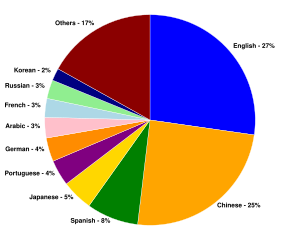
\includegraphics{InternetUsersByLanguagePieChart.svg.png}
\caption{Internet users by language \cite{InternetUsersByLanguagePieChart}.}
\end{figure}

\begin{table}[h]
\section{Table} % Adding a section was not verbally requested, but the example had it
\begin{center}
\begin{tabular}{ |c|c| }
English & 28\% \\
Chinese & 25\% \\
Others &  48\% \\
\end{tabular}
\caption{Top-3 languages on the internet}
\end{center}
\end{table}

\section{Referencing}
This is how we reference things
\bibliographystyle{plain}
\bibliography{refs}

\end{document}
